\section{Theory}








\subsection{Overlying Framework: {\normalfont \scshape RAMSES} and {\normalfont \scshape PHEW}}



%==============================
% RAMSES
%==============================



\subsubsection{{\normalfont \scshape RAMSES}}

\ramses\ is a N-body and hydrodynamical adaptive mesh refinement (AMR) code which uses the ``Fully Threaded Tree'' data structure of Khokhlov \parencite{FTT}. 
It simulates the time evolution of particles.
The domain is covered by a Cartesian grid, called the mesh.
Simulations require numerical integration, whose accuracy increases as the size of a grid cell decreases, but smaller grid cells naturally need more resources to cover a domain of the same size.
AMR is a method that ``\textit{tries to attain a fixed accuracy for a minimum cost}'' \parencite{AMR} by ``refining'' the mesh only where and when necessary.
``Refining'' in this case means that cells of smaller and smaller sizes are introduced until the desired accuracy is achieved.
Grid cells that contain lots of particles will be refined many times, while grid cells that contain no particles won't be refined at all.
The unrefined grid is called the ``\emph{coarse grid}'' and the number of times a cell of the coarse grid is refined is called the ``level of refinement''.
Cells which are not refined (any further) are called ``\emph{leaf cells}''.
They always have the highest level of refinement at their position.

The basic elements of the data structure in \ramses\ are groups of $2^{\text{dim}}$ sibling cells called ``\emph{octs}''.
Each oct belongs to a given level of refinement. 
All octs of a given refinement level are sorted in a doubly linked list, so each oct points to the previous and the next oct in the linked list of the particular level.
The fully threaded tree structure also demands that each oct points to the parent cell (the cell on the less refined level) as well as the $2 \cdot \text{dim}$ neighbouring parent cells and the $2^{\text{dim}}$ child octs on the next refinement level, assuming they exist. \\
%The cells on the least refined level are called the coarse grid. 
%To dynamically modify the AMR structure at each time step, first all cells are being marked for refinement according to user-defined criteria. 
%Any oct in the tree structure must be surrounded by $3^{\text{dim}}-1$ neighbouring parent cells, which enforces a smooth transition in spatial resolution.
Particles belonging to octs are organised in linked lists as well. 
A particle belongs to a particular oct if its position fits exactly into the oct boundaries, and all particles that belong to the same oct are linked together by a linked list. 
%Each oct can access the first particle of its linked list and the number of particles its list contains.

A system that contains many particles is called a ``N-body system''.
A collisionless N-body system is described by the following equations for the particles with position $\vec{x}_p$ and velocity $\vec{v}_p$:
	\begin{align}
		&\frac{\de\vec{x}_p}{\de t} =  \vec{v}_p &\frac{\de\vec{v}_p}{\de t} = - \nabla_x \phi 
	\end{align}
%
with
%
	\begin{align}
		 &\Delta_x \phi = 4 \pi G \rho \label{eq:poisson}
	\end{align}	
%
Where $\phi$ is the potential, $G$ the gravitational constant and $\rho$ the mass density field.
To compute the spatial movement of the particles, first $\rho$ is computed using a ``\emph{Cloud-In-Cell}'' (CIC) interpolation scheme.
The CIC scheme considers all particles to be cubes (``clouds'') of one cell size and of uniform density. 
The mass of a particle is deposited in cells based on what fraction of its ``cloud'' overlaps with the cell, thus determining the density field.
Once the density field is known, the Poisson equation (\ref{eq:poisson}) can be solved numerically and the potential $\phi$ is computed. 
Now the acceleration for each cell can be obtained, from which the particle acceleration $\tfrac {\de\vec{v}_p}{\de t}$ is computed using the inverse CIC interpolation. 
The acceleration is then integrated over time to compute the particle velocity $\vec{v}_p$ and position $\vec{x}_p$ using a second-order midpoint scheme.

%For a more detailed description of the code, I refer the reader to the release paper of \ramses\ \parencite{ramses}.

















%==============================
% PHEW
%==============================




\subsubsection{{\normalfont \scshape PHEW}} \label{chap:phew}

\phew\ is a structure finding algorithm implemented into \ramses. 
It is a ``watershed-based'' algorithm: ``\textit{These algorithms assign particles or cells to density peaks by following the steepest gradient, resulting in the so called `watershed segmentation' [...] of the negative density field.}'' \parencite{PHEW}.
%In the case of \ramses, \phew\ is applied to the mass density field defined by the projection of the particles' mass on the mesh.
\phew\ groups cells together by separating the mass density field along minima, thus dividing the density field into patches.
The density field is obtained with the deposition of the particle's mass on the mesh through CIC interpolation.
The algorithm can be divided in four main steps: segmentation, connectivity establishment, noise removal and substructure merging. 

In the first step, namely the ``watershed'' segmentation, the cells of interest are identified. % and their neighbours stored. 
%on the mesh are grouped together into patches around a local density maximum called the peak. 
These are all leaf cells which have a density above an user-defined density threshold and are called ``\emph{test cells}''.
If a cell doesn't have a denser neighbour, it is marked as a local density peak and assigned a peak label.
The peak label of a cell defines what peak patch this particular cell belongs to.\\
Then each cell copies the peak label from its densest neighbour.
This way, each cell is assigned to the peak ``closest'' to it by following the path of rising density. 
All test cells assigned to a particular peak form the aforementioned peak patch.
The separating surface between peak patches will be cell borders which contain local density minima, corresponding to the watershed analogy.

%In order to perform this segmentation, all leaf cells which have a density above an user-defined density threshold are marked. 
%These cells are called "test cells". 
%The neighbour cell with the highest density of each test cell is stored. 


%The test cells are then sorted by decreasing density and each cell copies the peak label from its most dense neighbour.
%Because the cells have previously been sorted, their densest neighbour will always have a peak label: Either it was a peak to begin with, or it has been accessed before because it is more dense.


In the next step, the connections between the peak patches need to be established. 
All test cells are examined for neighbours that belong to another peak. 
If a neighbouring cell with a different peak label is found, the density of the common surface between those two neighbours is defined as the average of these two cell densities.
%Obviously the connecting surface between two peak patches can consist of (surfaces of) multiple cells. 
The maximal surface density between two particular peak patches is considered as the ``\emph{saddle}'' between these two. 
Naturally, a peak patch can have multiple neighbouring peak patches. 
Out of all the saddles of all the neighbouring peak patches, the one with the highest density is called the ``\emph{key saddle}'' and the neighbour it connects to is referred to as the ``\emph{key neighbour}''.

The third main step, noise removal, requires a clear definition of what is to be considered noise. 
In \phew, each peak patch is assigned a value representing the contrast to the background called ``\emph{relevance}''.
A peak patch's relevance is defined as the ratio of the peak's density to its key saddle. 
A peak patch is considered noise if the its relevance is lower than a user-defined relevance threshold.
An irrelevant peak patch is then merged to its key neighbour. 
If an irrelevant peak patch doesn't have a key neighbour because it is isolated, it is discarded.



Expressed explicitly, merging a peak patch $i$ into a peak $j$ means that all cells of $i$ inherit the peak label of $j$.
%Due to these conditions, just like the test cells in the watershed segmentation step, the peaks are sorted by decreasing peak density in order to enable the propagating peak labels to travel as far as possible in one loop.
%In order to perform the noise removal, like in the segmentation step with the test cells, all peaks are sorted by decreasing density.
%This sorting makes sure that the noise removal can be executed in one loop only. 
Both peaks' saddles are merged as well: 
The peak patch $j$ inherits the saddles that connected $i$ to other patches.
Therefore, after two peaks are merged, new key saddles and the relevance need to be determined for the peak patches that have undergone merging.
%introduce loop here fso you don't have to later
%To maximise performance, the merging step is executed in a loop on peak patches sorted by decreasing density. 
This concludes the noise removal, since all irrelevant patches are either merged into relevant peaks or discarded.\\
%
%The last main step of the algorithm is merging of the peak patches.
As mentioned before, \phew\ can work in parallel on multiple processors.
The parallel implementation will be discussed in more detail in section \ref{chap:parallel}.
In order to produce unique results when executed on multiple processors, the merging of peak patches needs to obey the following three rules:
%
\begin{enumerate}
	\item Whether a peak should be merged into its key neighbour or not is determined by some criterion.
	\item A peak patch is only merged into its key neighbour.
	\item The peak of the key neighbour must have a higher density.
\end{enumerate}
%
In the case of noise removal, the criterion is to satisfy the relevance condition. The criterion is different for the substructure merging step.\\
%
Once the noise removal step is completed, the remaining structure consists only of peak patches which satisfy the relevance condition and is referred to as ``\emph{level 0 clumps}''. 
These clumps represent the structure on the lowest scale.
A large halo for example, which can very roughly be described as ``a large clump'' in a first approximation, would be decomposed into many small clumps. In order to identify such a halo as a single object, one more step is necessary.


The identified level 0 clumps can be merged further into composite clumps.
The procedure used is exactly the same as in the previous step, only the merging criterion is different:
The new criterion is a threshold for the key saddle density. All peak patches whose key saddle density is \emph{higher} than the user-defined threshold are merged into their key neighbour.
The saddle threshold defines which clumps should be considered as separate structures and which should be  merged and considered as composite structures.\\
%
After the first round of merging, the lowest level of structure has been merged into first composite clumps.
If clump $a$ is merged into clump $b$, then $b$ is called the ``\emph{parent}'' of $a$.
Because of the merging, again the lists of saddle points change for the ``surviving'' clumps, and the list as well as the key saddles need to be updated.
The peak labels of the cells however are not updated in this merging procedure: 
They are necessary to preserve the information on substructure.
Only the clump properties like volume, mass, position and neighbours are merged.\\
%
The merging of clumps creates connections between peak patches where there were none before in the sense that the surviving peak patches can establish a connection to other surviving patches because clumps between them were merged into them.
See for example in figure \ref{fig:phewlevels}: The red and the blue clump establish a connection after all the smaller clumps between them have been merged into them in the span of two merging loops.
Each merging loop then represents a different level of substructure:
In each loop, greater structures are being merged into each other than there were in the loop before.
Starting from the lowest level, which are the peak patches identified after noise removal, clumps are merged into each other until none satisfy the merging criterion any more.
%Figure \ref{fig:phewlevels} illustrates the concept of the described merging hierarchy.
%

\begin{figure}[htbp]
%\parpic[r]{%
\centering
	\fbox{
		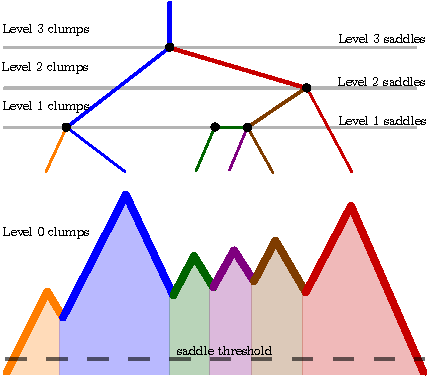
\includegraphics[width = 9.5cm, keepaspectratio]{images/phew/saddle_hierarchy2.pdf}
	}
	\caption{
		Hierarchy of clumps as created by \phew's clump merging algorithm. 
		Level $n$ saddle points are used for merging during the $n-$th round of merging. 
		A peak patch is always merged into its key neighbour and it is only merged into a peak patch with a higher density.
		In this figure, the merging criterion is that the key saddle is higher than the saddle threshold.\\
		Image adapted from \cite{PHEW}}
	\label{fig:phewlevels}
\end{figure}
%

When the merging is finished, the clumps have been merged into the largest possible structures that satisfy the relevance and saddle density conditions.
The remaining structures are large clumps and they are considered as halos, provided that the clumps are massive enough.
A halo must have a minimal mass that can be set by the user.\\
%
The label of halos will be the label of clumps which are never merged into an other, but only have other clumps merged into them. 
Such clumps are called ``\emph{halo-namegivers}''.



In summary, \phew\ identifies halos by the following three criteria:
\begin{itemize}
	\item {Halos are composed of cells with densities above a density threshold.}
	\item{A halo must have a minimal mass that can be set by the user.}
	\item {Within a halo, the subhalos are peak patches that are relevant, i.e. aren't considered noise. Their edge is determined by local density minima surfaces.}
	\item {If the interface between two relevant peak patches is less dense than a threshold (saddle threshold), the two peak patches are considered to be two independent halos.}
\end{itemize}




%Since \ramses\ is a parallel code which uses the MPI library and the fundamental strategy of splitting the computational domain between MPI tasks, \phew\ must be able to work in parallel on the split domain as well.
%This is not a trivial task since the watershed segmentation is non-local by nature.
%This concludes the description of the way \phew\ works. 
%I will describe the parallel implementation of \phew\ (and \ramses) briefly and simplified in the following section, while focussing on the parts and tools necessary for the unbinding code. 
%For a more detailed description of \phew\, I refer the interested reader to its release paper \parencite{PHEW}.

%Splitting the computational domain between multiple MPI tasks is realised by introducing virtual boundaries.
%Instead of having data of the whole computational domain, each MPI task has only the knowledge of its own part of the domain.
%Around the computational domain of each MPI task, there is a so called "virtual domain". 
%All necessary data from other MPI tasks is communicated with MPI tools into the so called virtual domain, which surrounds the "real domain", so that the virtual domain mimics what happens in the domains of other tasks.
%This way, only the necessary information needs to be transferred and the code can be executed on distributed memory computers.




%\ramses\ advances the timely evolution of the particles timestep by timestep, thus creating a snapshot of the particles' position and velocity at each timestep. 
%\phew\ can then be executed on the results of the time advancement, meaning that the segmentation is only performed on snapshots of the simulation. 
%This yields the segmentation of the density field into patches at every timestep (that is on every required timestep that would be stored as output), but the patches found can't be tracked trough time:
%Only one more or one fewer local density maximum would shift all peak indices by which the peaks are labelled. 
%
%The peak patches correspond in the case of particles to spatially separated regions with a density higher than a given density threshold.
%Such regions are commonly referred to as \emph{clumps} of particles and \phew\ is also called a \emph{clumpfinder}.
%


















\subsubsection{Parallel implementation}\label{chap:parallel}

\ramses\ is a parallel code which makes use of the MPI library.
The use of MPI (message passing interface) allows a process on a distributed memory architecture to be executed in parallel by multiple tasks and enables various types of communications between them.
 
The fundamental parallelisation strategy used in \ramses\ is domain decomposition,
where a part of the total spatial computational domain is assigned to each processing unit, or ``MPI task''.
It makes use of the fact that most calculations on grids do not require the knowledge of the entire computational domain, but only the cells in their vicinity
The basic idea of the domain decomposition is illustrated in figure \ref{fig:parallel}, where a 2D-grid is split between two processors. 
The partial domains do not overlap and a thin layer of cells called the ``\emph{virtual boundary}'' is introduced where the domain was cut. 
Necessary information is then communicated across MPI tasks from the other tasks' ``real domain'' into the virtual boundary, so that the virtual boundary copies what happens in the domains of other tasks and allowing the execution of the code as if the domain wasn't split.
Two tasks working on the same problem allows a much faster execution time, but it also enables the solution of a much bigger problem that only one task couldn't do on its own, e.g. because of memory restrictions.

\begin{figure}[htbp]
	%\parpic[r]{%
	\centering
	\fbox{
		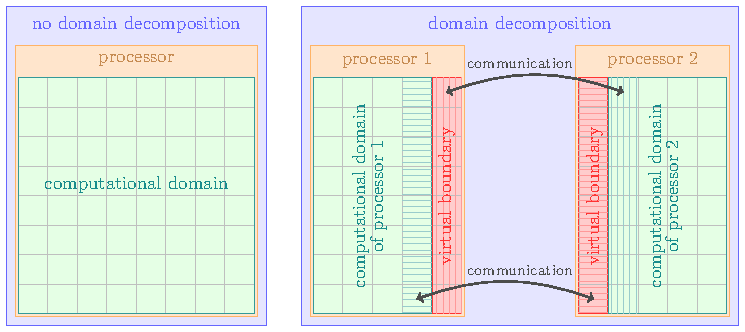
\includegraphics[width = 12.5cm, keepaspectratio]{images/tikz/parallelisation.pdf}
	}
	\caption{
		The basic idea of domain decomposition. Here a 2D-grid is split between two processors (right) instead of only one (left). 
		The partial domains do not overlap and where the domain was cut, a  ``virtual boundary'' is introduced. 
		Necessary information is then communicated between processors from the other tasks' ``real domain'' into the virtual boundary, so that the virtual boundary copies what happens in the domains of other tasks and allows the execution of the code as if the domain wasn't split.
	}
	\label{fig:parallel}
\end{figure}




\phew\ uses the virtual mesh boundary as well, since every cell on each domain must have the information of all its neighbours.
%by shifting the local peak index to an interval of indices reserved only for one particular task.
%The reserved interval is determined by the number of peaks found by all tasks.
%Every task has an interval of peak indices reserved for itself, making the global peak index unique.
%During the segmentation loop, all cells that change their peak patch label are counted. 
%The segmentation step, which is executed in a loop, is repeated until there are no more changes of peak labels of cells on the entire computational domain.
%The peak patch labels in the virtual boundary
%are updated using MPI communications before every loop.\\
%
Initially, all peaks are counted and their number is communicated throughout all MPI tasks.
This gives all MPI tasks the knowledge of the total number of peaks of the entire computational domain, allowing the introduction of a peak label that is globally unique for each peak. 

Similarly to the virtual mesh boundary, a virtual peak boundary is necessary.
For the peak patch merging step, each peak patch on each task's domain needs the information of the peak patches that surround it.
If, for example, a peak patch is split in two by the domain boundaries between two tasks, both tasks need to know all the peak patch's neighbours on the other task's domain.\\
%
Unlike the mesh boundary however, the virtual peak boundary is not a fixed region in space.
Because of the merging, peaks gain neighbours they hadn't had before.
This requires that new peaks are introduced to the virtual peak boundary during the merging procedure.
%Virtual peaks are introduced by assigning them a local peak index.
%Each tasks stores the virtual peaks in the first free place in the memory after the ``real'' peaks.
Once introduced, all other peak properties, e.g. its relevance and saddle points, can be transferred by means of MPI communication.

The virtual peak boundary requires two types of communications. 
One type is the collection (sum, minimum or maximum) of a value for a peak from all tasks which have that particular peak patch in their virtual boundary to the owner of the peak.
The ``\emph{owner}'' of the peak is the task where the density peak is in the ``real'' domain, as opposed to the virtual mesh boundary.
Imagine for example the calculation of a peak patch's total volume on multiple tasks: 
Each task would compute the volume of that peak patch on its own domain and then all these partial results would be sent to the peak's owner and summed up.\\
%
In that scenario only the peak's owner has the total volume of the patch, but the ones that have it in their virtual boundary still only have their partial values.
This brings us to the second required type of communication:
A scatter of data from the owner of the peak to all tasks with that particular peak in their virtual boundary. 
In our example, the owner of the peak would send the computed total volume of the peak patch to all the tasks which require that information. 
%In this case, the value of the boundary peaks is overwritten by the new data.\\
%
In order to perform these communications, a communication structure (called the ``peak communicator'') must be built first. 
The purpose of the peak communicator is to establish how many peaks of every task are owned by any other task, or in other words: ``what needs to be sent (and received from) where''.
Once that is known, the communications between the processes and thus the parallel merging can be performed.



The following summary of results and tools available after the execution of the segmentation algorithm concludes this brief description of \phew\ and \ramses:
%
\begin{itemize}
	\item A list of peak patches, composed of overdense leaf cells, representing clumps of particles
	\item A hierarchy of these clumps, established during the merging of the peak patches
	\item A virtual boundary for cells and another virtual boundary for peak patches along with as a set of communication tools which enable the transfer of peak patch information across MPI tasks.
\end{itemize}



%Now that the N-body and the segmentation algorithms are introduced, I would like to discuss in the next section what `unbound' particles are.























%======================
%Unbinding
%======================





\subsection{Unbinding Particles}



\subsubsection{Constraints and Limitations}

%In this section I will discuss what conditions need to be satisfied in order for a particle of mass $m_p$ and velocity $\vec{v}_p$ to be considered as "bound".




%I will discuss the physical meaning of eq. \eqref{eq:bound} later.
%First I need to establish what assumptions I make and how I describe the system of particles in order to gain an expression for the energy $E$ which can be interpreted and calculated.



Due to complexity and size, solutions of physical problems often require simplifications and assumptions to be made.
In this section, the assumptions necessary for the unbinding algorithm are explained shortly.

Firstly, the situation under consideration is assumed to be \emph{time-independent}.
This allows an easy description of the system by introducing local energy conservation on one hand, but on the other hand, the information necessary for a time-dependent description is not readily obtainable.
\ramses\ computes the evolution of the particles time step by time step, thus creating a snapshot of the particles' position and velocity at each time step. 
%The particles represent collisionless dark matter particles.
\phew\ can then be executed on the results of the time advancement, meaning that the segmentation is only performed on snapshots of the simulation. 
%This yields the segmentation of the density field into patches at every time step (or rather on every required time step that would be stored as output).
In order to obtain the information necessary for a time-dependent description, the entire simulation from beginning to end must be known, which contradicts the requirement for on-the-fly analysis.
Furthermore, due to the nature of \phew, the found peak patches can't be tracked trough time:
Only one more or one fewer local density maximum would shift all following peak labels.
%This leads to the first restriction: I must consider the system to be \emph{time independent}. 


The purpose of a particle unbinding algorithm is to determine for each particle of a (sub)structure if the particle is bound to that particular structure. 
%, which means to determine if it satisfies the condition (\eqref{eq:bound}) or not.  
The focus on the substructure itself, as opposed to a global perspective, leads to the second used simplification: 
The structure is considered to be \emph{isolated}.
Any effects on the particles that arise from outside the structure that is being investigated, e.g. tidal effects, are neglected.
(Some consequences of neighbouring structures will be accounted for, which is will be discussed in section \ref{chap:neighbours}).
This simplification is also motivated by the enormous computational expense that would arise from taking the entirety of structures in the computational domain into account for each substructure anew.

Lastly, a third major simplification is used.
As will be introduced more properly in the following section, whether particles are bound to a clump depends on the gravitational potential of the clump itself.
In classical mechanics, the gravitational potential $\phi(\vec{r})$ is determined by the poisson equation \ref{eq:poisson}.
%%
%\begin{align}
%	\Delta \phi(\vec{r}) = 4 \pi G \rho(\vec{r}) \label{eq:poisson}
%\end{align}
%%
%where $\Delta$ is the Laplace operator, $G$ is the gravitational constant and $\rho$ is the mass density field. 
It represents the amount of work needed to move the particle from infinity (where as a point of reference the potential is usually chosen to vanish) to the place it is.\\
%
In theory, equation \ref{eq:poisson} can be solved, because if all the particle positions are known, then the density field $\rho$ is known as well.
Sadly the solution for each particle depends on each other particle, so calculating it makes it a computationally expensive code of order $\mathcal{O}(N^2)$.
This is not acceptable for a code required to work on-the-fly.
Instead, an analytical solution which is valid for \emph{spherically symmetric} systems is used.
%Consider a spherically symmetric clump of radius $r_{max}$ such that there are no more particles further away from the centre of mass than $r_{max}$ and total mass $M_{tot}$.
It is a bit unfortunate to introduce the assumption of spherical symmetry, because \phew\ had no need for it and was able to identify clumps of any shape, an information which is ignored at this point.
Nonetheless, due to the lack of a better solution at this time, it was a necessity.





To summarise, each substructure clump as found by \phew\ is considered to be an isolated, time independent spherical system of collisionless dark matter particles.



















\subsubsection{Bound Particles}

In general, one can assign every particle a total energy $E$. 
A particle is considered to be ``\emph{bound}'' if
%
\begin{align}
	E < 0 \label{eq:bound}
\end{align}
%
or ``\emph{unbound}'' if it doesn't satisfy this condition.
%In order to determine an expression for the total energy $E$ of a particle, one must first establish the manner in which the system of particles will be described, particularly which assumptions are made.
%The assumptions, on the other hand, are influenced by the system to be described, but also by the result one is trying to achieve.
%So we need to have a look at ``what we have'' and ``what we want''.

Consider now an isolated clump that is made up of $N$ particles, where the position $\vec{x}_i$, the velocity $\vec{u}_i$ and the mass $m_i$ of every particle $i$ is known. 
Even though the system is assumed to be time independent, the structures within the system do not need to be stationary.
On the contrary: The clumps are expected to be in motion with respect to the computational grid.
It is often useful to consider the problem in another frame of reference, namely the ``centre of mass'' frame.
The centre of mass of a clump of $N$ particles is defined as:
%
\begin{align}
	\vec{x}_{CoM} = \frac{\sum_{i=1}^{N} m_i \cdot \vec{x}_i}{\sum_{i=1}^{N} m_i} \label{eq:com}
\end{align}
%
%Where $N$ is the number of particles of the clump. 
The centre of mass frame is then defined as the frame of reference where the velocity of the centre of mass (also called the ``\emph{bulk velocity}'') vanishes:
%
\begin{align}
	\vec{v}_{CoM} = \frac{\de}{\de t} \vec{x}_{CoM}  = \frac{\sum_{i=1}^{N} m_i \cdot \vec{u}_i}{\sum_{i=1}^{N} m_i} \equiv 0 \text{ \hspace{5mm} in centre of mass frame} \label{eq:vcom}
\end{align}
%
and the centre of mass is at the origin:
%
\begin{align}
	\vec{x}_{CoM} \equiv 0
\end{align}
%
The particle positions and velocities in the centre of mass frame are then
%
\begin{align}
	\vec{x_i}\ ' &= \vec{x_i} -\vec{x}_{CoM} \equiv r_i\\
	\vec{u}_{i}\ ' & = \vec{u}_i - \vec{v}_{CoM} \equiv \vec{v}_i \text{\hspace{1cm} with \hspace{1cm} }  v_i \equiv ||\vec{v}_i|| = \sqrt{v_{x,i}^2 + v_{y,i}^2 + v_{z,i}^2}
\end{align}
%

The assumption of time-independence and isolation allow to describe the clump by means of classical mechanics.
In such a system the energy $E_i$ of a particle $i$ in the centre of mass frame of the clump it belongs to can be expressed as 
\begin{align}
	E_i = T_i + V_i = \frac{1}{2} m_i \cdot v^2_i + m_i \phi (\vec{r}_i)\label{eq:E}
\end{align}
%
and is conserved:
\begin{align}
	E_i = const
\end{align}
Where $T_i = \tfrac{1}{2}m_p v_i^2$ is the \emph{kinetic energy} and $V_i = m_i \cdot \phi(\vec{r}_i)$ is called the \emph{potential energy} of the particle. 
$\phi(\vec{r}_i)$ is called the \emph{potential}.
%The expression for $\phi$ is discussed in the next section.
%In scope of this section, it suffices to note that $\phi \leq 0$ .

Plugging equation \eqref{eq:E} into the condition for a particle to be bound \eqref{eq:bound}, we get
%
\begin{align}
	\frac{1}{2} m_i \cdot v_i^2 + m_i \phi(\vec{r}_i) < 0
\end{align}
%
Or equivalently:
%
\begin{align}
	v_i < \sqrt{- 2 \cdot \phi(\vec{r}_i)} \label{eq:boundv}
\end{align}
%
These equations allow for an evident physical interpretation of the criterion for a particle to be bound:
It is bound if its kinetic energy is lower than the absolute value of the (gravitational) potential that it experiences. 
A bound particle's movement will be constrained by the potential:
The potential will always pull the particle towards the centre of mass of the clump. 
It can not escape arbitrarily, but will orbit the clump on elliptic trajectories.
%Equation \eqref{eq:boundv} also leads to the definition of the escape velocity $v_{esc}$:
%
%\begin{align}
%	v_{esc} = \sqrt{-2 \phi} \label{vesc}
%\end{align}
%
%Which is the minimal velocity a particle needs to have for it not to be bound to the clump.
%Equivalently to equation \eqref{eq:boundv}, a particle is considered bound if:
%\begin{align}
%	v < v_{esc}
%\end{align}
%%
%Or to put it in simple words: A particle is considered bound if it cannot escape the spatial boundaries of the potential that it experiences. 


$\vec{r}_i$ and $\vec{v}_i$ are known for each particle.
What remains to be found is an expression for the potential $\phi$.
Since only isolated collisionless dark matter particles are considered, the potential that influences the particles is the gravitational potential of the particles themselves.
In a spherically symmetric system, the potential at each point is determined by the absolute (radial) distance as opposed to its exact location.
Thus the potential can be expressed in the clump's centre of mass frame as $\phi(\vec{r}_i) = \phi(d_i)$ with 
\begin{align}
	d_i = \sqrt{(r_{i,x}-x_{CoM,x})^2 + (r_{i,y}-x_{CoM,y})^2 + (r_{i,z}-x_{CoM,z})^2}
\end{align}

The spherically symmetric Poisson equation (eq. \ref{eq:poisson}) can be solved for $\phi$:
%
\begin{align}
	\phi (r_i) &=  - G \int\limits_{r_i}^{r_{max}} \frac{M(<\tilde{r})}{\tilde{r}^2} \mathrm{d}\tilde{r}
	- G  \frac{M_{tot}}{r_{max}}
	\label{eq:sol_phi}
\end{align}
%
Where $M(<r) \equiv \int\limits_0^r 4 \pi \rho(\tilde{r})\tilde{r}^2 \mathrm{d}\tilde{r} $ is the mass enclosed by a sphere of radius $r$ such that the clump's total mass is enclosed by the radius $r_{max}$: $M_{tot} = M(<r_{max})$.
The full derivation of equation \eqref{eq:sol_phi} is given in appendix \ref{app:sol_phi}.


%The general idea is to simplify the poisson equation (eq. \eqref{poisson}) by assuming spherical symmetry of the problem and then solving the equation with an assumed density function $\rho (r)$.



















\subsubsection{Accounting for Neighbouring Structures}\label{chap:neighbours}

The boundaries of a particle's trajectory in a given potential $\phi$ can be estimated using the conservation of energy:
%
\begin{align}
	E/m_p = \frac{1}{2} v^2 + \phi = const.
\end{align}
%
A gravitational potential is qualitatively shown in figure \eqref{fig:orbits} as well as a particle $\alpha$ with $\frac{1}{2}v^2 < - \phi$.
The total energy per particle mass $E/m_p$ of the particle on the graph is then exactly the difference between the negative potential and the kinetic energy on the $y$-axis.
In order to conserve energy, the curve of possible kinetic energies (dotted line in figure \ref{fig:orbits}) that the particle may take on will always have the same distance $E/m_p$ from the negative potential curve.
Because $v^2\geq 0$, the spatial boundaries of a particle's trajectory can be found by following the curve of possible kinetic energies of the particle to the point where $v^2 = 0$.

\begin{figure}[h!]
	\centering
	\minipage[t]{0.45\textwidth}
	%\centering
	\fbox{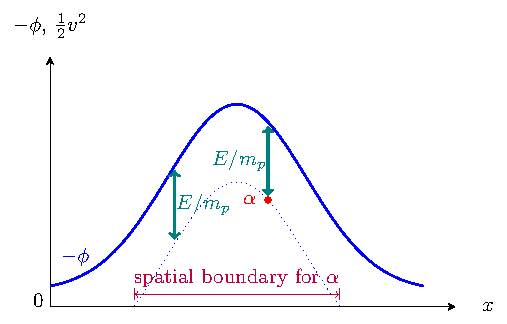
\includegraphics[height=4.45cm, keepaspectratio]{images/tikz/boundaries.pdf}}%
	\caption{A qualitative plot of a potential $\ -\phi$ and a particle $\alpha$. 
		The boundaries of the particle's trajectory can be found using energy conservation $E/m_p = \frac{1}{2}v^2 + \phi$ by following the curve of the particle's kinetic energies (dotted line) to the points where $v^2=0$.	
	}%
	\label{fig:orbits}
	\endminipage%\hspace{.1cm}
	\hspace*{\fill}
	%
	\minipage[t]{0.55\textwidth}
	%\centering
	\fbox{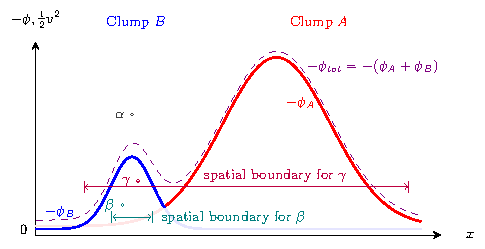
\includegraphics[height=4.45cm, keepaspectratio]{images/tikz/potentials.pdf}}%
	\caption{Qualitative potential of a halo containing two clumps $A$ and $B$. Three particles assigned to $B$ are shown: $\alpha$ is not bound to $B$, $\beta$ is bound, $\gamma$ satisfies the energy condition to be bound, but can wander off into clump $A$ and shouldn't be considered as such.
	}%
	\label{fig:potentials}
	\endminipage\hspace*{\fill} 
\end{figure}
%
This fact changes the situation significantly for the interpretation of what particles should be considered bound as follows.
Consider now an isolated halo that consists of two clumps, $A$ and $B$, where $B$ is a smaller clump nested within clump $A$.
Their potentials are qualitatively depicted in figure \eqref{fig:potentials}. 
Three particles assigned to $B$ with different kinetic energies are marked, representing three different cases:
%
\begin{itemize}
	\item Particle $\alpha$ has a kinetic energy higher than the potential, it is clearly not bound to the clump $B$.
	\item Particle $\beta$ has a kinetic energy lower than the potential at that distance from the centre of mass, so it will remain bound on an elliptic trajectory around the centre of mass.
	\item Particle $\gamma$ is considered energetically bound to the clump just like $\beta$, i.e. it satisfies the condition \eqref{eq:boundv}, but it won't necessarily remain on an elliptic trajectory around clump $B$'s centre of mass: Because of clump $A$'s neighbouring potential, the particle can leave the boundaries of clump $B$ and wander off deep into clump $A$.
\end{itemize}
%

These considerations show that due to the fact that subhalos will always have neighbouring structure, there will be particles like $\gamma$ that can wander off into neighbouring clumps even though they satisfy condition \eqref{eq:boundv}.
It is obvious that particles like $\gamma$ shouldn't be considered as bound and that therefore the bound condition needs to be modified appropriately.
Even though the clumps were assumed to be isolated, clumps that make up substructure will always have at least one neighbour by their nature.
The reason $\gamma$ can wander off is because its boundary extends past the interface that connects the two clumps, so the condition for a particle to be bound must be that its trajectory must never reach that interface.
Defining $\phi_S$ to be the potential of clump $B$ at the interface to the neighbouring structure that is closest to $B$'s centre of mass, the condition for a particle to be bound \emph{exclusively} to a particular clump can be written as
%
% Need energy to be ``more negative'' !
\begin{align}
	E/m_p = \frac{1}{2}v^2 + \phi -  \phi_S < 0
\end{align}
%
or equivalently:
%
\begin{align}
	v < \sqrt{ - 2(\phi - \phi_S) } \label{eq:boundv_corr}
\end{align}


According to the argumentation above and figures \ref{fig:orbits} and \ref{fig:potentials}, it is to be expected that demanding particles to be exclusively bound will find more unbound particles than not doing so, where particles close to the centre of mass should be more likely to be exclusively bound than the particles closer to the edge of the subhalo.












\subsubsection{Structure Hierarchy: What to Do With Unbound Particles}

One last thing that needs to be considered with respect to unbinding particles is the hierarchy of substructures that is found by \phew, as described in section \ref{chap:phew}.
As mentioned before, for conventional reasons, it is assumed that all particles within a halo are bound to the halo. 
Therefore there is no need to examine the halo-namegiver clumps for unbound particles.\\
The situation is different for substructure clumps:
%All particles assigned to a halo-namegiver clump are assumed to be bound to it.
If a particle is found to be not bound to a clump, it shouldn't be discarded or removed from the entire structure, but passed on to the next higher level of substructure for examination. 
%Therefore, the unbinding of particles needs to be executed starting on the lowest level of clumps, namely the level 0 clumps, and work its way up to the top level of each structure.
This way as much as possible information on substructure is preserved and the unbinding procedure ends naturally when the level of the halo-namegiver clumps is reached.

















\subsubsection{Biased Clump Properties}\label{chap:iter_theory}

The last attempt to improve the unbinding algorithm is to take into account that the properties of the found substructure are biased.
Consider this very simplified case: A known spherical halo contains exactly one, also spherical and known, subhalo.
Such a situation can be seen in figure \ref{fig:dice_two_origin}.
By construction, the clumpfinder \phew\ will not recognise these two as two spherical clumps. 
Instead, it will group cells by following the steepest density gradient.
(The clumps that \phew\ actually finds can be seen in the top row of fig. \ref{fig:dice_two_results}.)
In consequence, the clump properties, e.g. the centre of mass and the bulk velocity, based only on particles that are found to be a part of the clump will differ from the known properties for two reasons:
%
\begin{enumerate}
	\item Some of the particles that are known to be a part of the subhalo will be assigned to the halo instead.
	The found subhalo will have missing particles.
	\item The subhalo is nested within the halo.
	It will be contaminated by the halo's particles. 
\end{enumerate}
%
So in order to retrieve clump properties that are closer to the known properties, some further work needs to be done.
It seems likely that the clump properties after particle unbinding should be closer to the known ones, particularly so if neighbouring structures were taken into consideration and therefore the remaining structure contains only exclusively bound particles.
A possible improvement is to recompute the clump properties after unbinding and use this updated information to go through the entire procedure again.
The whole unbinding procedure is reiterated until the bulk velocity of each clump converges.
The bulk velocity is considered converged when the relative difference of the old and the new bulk velocity is smaller than a user-defined convergence limit $\varepsilon$:
\begin{equation}
\text{bulk velocity converged} \Leftrightarrow \left | \frac{v_{bulk,old} - v_{bulk,new}}{v_{bulk,new}} \right | < \varepsilon
\end{equation}


This concludes the detailed description of the requirements of the unbinding algorithm. 
In the following chapter, its implementation is described.